\documentclass{llncs}
\usepackage{amsfonts}
\usepackage{amsmath}

\usepackage{tikz}
\usepackage{tkz-graph}

\DeclareMathOperator*{\argmin}{arg\,min}

\begin{document}

\title{CP-Based Local Search for Minimum Cost Linear Extension}

\author{T.O. Bonates \and L.F.S. Oliveira \and L.V. Oliveira \and P.C.L. Silva}

\institute{UFERSA}

\maketitle

\abstract{Breve descri\c{c}\~ao do modelo CP para busca local. Pode ser usado para CPAIOR 2013, ou apenas na nova vers\~ao do artigo completo.}

\section{Introduction}

Let $E$ be a $n$-set and let us write $E=\{x_1,\ldots,x_n\}$. A partially ordered set (or simply, a \emph{poset}) defined on $E$ is a pair $\mathbf{P}=(E,\leq)$, where $\leq$ is a binary relation on $E$ that is transitive, reflexive and antisymmetric, \emph{i.e.}, $\leq$ is a binary relation satisfying, respectively:

\begin{enumerate}
\item[(i)] $x_i \leq x_j, \;\; x_j \leq x_k \; \Rightarrow \; x_i \leq x_k, \;\; \forall \: x_i, x_j, x_k \in E$;
\item[(ii)] $x_j \leq x_i, \;\; \forall \: x_i \in E$;
\item[(iii)] $x_i \leq x_j, \;\; x_j \leq x_i \; \Rightarrow \; x_i=x_j, \;\; \forall \: x_i,x_j \in E$.\\
\end{enumerate}

In a partial order $\mathbf{P}=(E,\leq)$ there might exist pairs of elements $x_i,x_j \in E$, with $x_i \neq x_j$, such that we have neither $x_i \leq x_j$ nor $x_j \leq x_i$ in $\mathbf P$. Two elements $x_i,x_j$ of a poset $\mathbf P$ are said to be \emph{comparable} if $x_i \leq x_j$ or $x_j \leq x_i$ in $\mathbf{P}$; otherwise, they are said to be \emph{incomparable}, which is denoted by $x_i \sim x_j$. We say that $x_j$ \emph{covers} $x_i$ in $\mathbf P$ if $x_i < x_j$ and if there is no element $x_k$ in $\mathbf P$ satisfying $x_i < x_k < x_j$.\\

A linear extension of a poset $\mathbf{P}=(E,\leq)$ is a permutation $\mathbf{L}$ of the elements of $E$ such that $x_i$ comes before $x_j$ in $\mathbf{L}$ whenever $x_i < x_j$, for all comparable pairs $x_i,x_j \in E$. It is a well-known fact that every poset admits at least one linear extension (see, {\it e.g.}, \cite{Stanley}). Let us write a linear extension $\mathbf{L}$ of poset $\mathbf{P}$ as
\[
{\mathbf L}=\left( x_{i_1}, x_{i_2} , \ldots, x_{i_n} \right) \in E^n,
\]
\noindent with $x_{i_1} <_{\mathbf L} x_{i_2} <_{\mathbf L} \ldots <_{\mathbf L} x_{i_n}$. It is typical for a poset to admit more than one linear extension. Thus, it is natural to consider an optimization problem that asks for the best linear extension of a poset $\mathbf P$, according to some criterion.\\

Let $c: E \times E \rightarrow \mathbb{R}_+$ be a cost function that associates a non-negative real value with every pair $x_i,x_j \in \mathbf{P}$, while satisfying the following conditions:

\begin{equation}
\left\{
\begin{array}{lll}
c(x_i,x_j)=0, & \mbox{if} & x_i \leq x_j;\\
0< c(x_i,x_j)< +\infty, & \mbox{if} & x_i \sim x_j;\\
c(x_i,x_j)=+\infty, & \mbox{if} & x_i>x_j.
\end{array}
\label{func} \right.
\end{equation}

We will write the total cost of a linear extension ${\mathbf L}=\left(x_{i_1} x_{i_2} \ldots x_{i_n}\right)$ as
\begin{equation}
\label{custo} \displaystyle c({\mathbf L})=\sum_{j=1}^{n-1}c(x_{i_j}, x_{i_{j+1}})
\end{equation}

Given a poset $\mathbf P$ and a cost function $c$ as described above, the Minimum Cost Linear Extension problem (thereby referred to as MCLE) asks for a linear extension $\mathbf L$ of $\mathbf P$ which minimizes $(\ref{custo})$. In other words, we are interested in finding $\mathbf{L}^*$ satisfying
\[
\mathbf{L}^* \:\in\: \argmin \{c(\mathbf{L}) : \mathbf{L} \mbox{ is a linear extension of } {\mathbf P} \}.
\]

The MCLE was originally defined in \cite{Liu} and further studied in \cite{Wu}.
In \cite{Liu} the authors showed that the MCLE
generalizes the so-called bump number and jump number problems on posets.
Specifically, if we define $c(x_i,x_j)=1$, for $x_i \sim x_j$, the problem becomes
equivalent to the jump number problem. Since the jump number problem is known to be NP-hard (see \cite{Bouchitte}), the MCLE is also NP-hard.
In this work, however, we concentrate on the general version of the problem, in
which $\mathbf P$ is an arbitrary poset and $c$ is an arbitrary non-negative real-valued cost function satisfying conditions (\ref{func}).


\section{Related Work}

Literature Review: essentially Liu1 and Liu2. Use of CP for local search.

\section{CP-Based Local Search for MCLE}

Given a linear extension $\mathbf{L}_0$ of a poset ${\mathbf P}=(E,\leq)$, with $E=\{x_1,\ldots,x_n\}$, we are interested in finding a linear extension $\mathbf{L}_1$ within a certain neighborhood of $\mathbf{L}_0$ such that $c(\mathbf{L}_1) < c(\mathbf{L}_0)$.\\

For the purpose of formulating the CP model for local search, we shall define a linear extension of poset $\mathbf P$ as a vector $e \in \{1,\ldots,2n+1\}^{n}$ satisfying:\\

\begin{itemize}
\item[(a)] $e_i \neq e_j$, $\forall i,j \in \{1,\ldots,n\}, i \neq j$;\\
\item[(a)] $e_i < e_j$, $\forall i,j \in \{1,\ldots,n\}$ with $x_i <_{\mathbf P} x_j$;\\
\end{itemize}

Let us define integer decision variables $V_i \in \{1,\ldots,2n+1\}$, for $i=1,\ldots,n$, with each $V_i$ corresponding to the position of the $i$-th element in the linear extension.
Conditions (a) and (b) above translate into the following constraints on the $V$ variables:\\
\begin{eqnarray}
&& \texttt{all-different}(V_1,\ldots,V_n) \label{C1}\\
&& V_i < V_j, \; \forall i,j \in \{1,\ldots,n\} \mbox{ such that } x_i <_{\mathbf{P}} x_j.\label{C2}
\end{eqnarray}

For any instantiation of $V$ satisfying constraints (\ref{C1}) and (\ref{C2}), let us define $s_k$ as the index of the $k$-th order statistic of $\{V_1,\ldots,V_n\}$, for $k=1,\ldots,n$. Clearly, the sequence $\left(x_{s_1}, x_{s_2}, \ldots, x_{s_n}\right)$ is a linear extension of $\mathbf P$, to which we shall refer as the linear extension \emph{induced} by $V$.\\

Let $\mathbf{L}_0=\left(x_{i_1}, \ldots, x_{i_n}\right)$ and let us define $p \in \{1,\ldots,2n+1\}^n$ with $p_{i_j}=2j$, $j=1,\ldots,n$. Let us also define $\mathbf{L}_1$ to be the linear extension induced by the vector $V$ of decision variables. In order to detect which elements $x_j$ ($j=1,\ldots,n$) of $E$ change their positions in $\mathbf{L}_1$ with respect to $\mathbf{L}_0$, we can write the reified constraint:
\begin{eqnarray}
&& \left| V_j - p_{i_j} \right| > 1 \Leftrightarrow D_j,
\end{eqnarray}

\noindent where each $D_j$ is a binary (Boolean) decision variable corresponding to whether or not the position of $x_j$ in $\mathbf{L}_1$ differs from that in $\mathbf{L}_0$.\\

By constraining the number of variables $D_j$ that take value $1$ to be at most $w$ we restrict the CP model to explore a neighborhood around $\mathbf{L}_0$, namely the set comprised of linear extensions in which at most $w$ elements of $E$ change their positions with respect to $\mathbf{L}_0$. The parameter $w$ will be called the \emph{width} of the neighborhood, which will be denoted by $N_w(\mathbf{L}_0)$. We shall thus write
\begin{equation}
\sum_{j=1}^n D_j \leq w.
\end{equation}

Note that we allow the model to slightly change the absolute position of each element $x_j$, without causing $D_j=1$. The reason for this is that changing the absolute position of $x_j$ by a single unit is not enough, by itself, to change $x_j$'s relative position with respect to the remainder of the extension. It is interesting, however, to allow for such a change, since moving $x_j$ one unit forward can make room for another element to occupy $x_j$'s former position in $\mathbf{L}_0$. Figure \ref{Movement} illustrates such a scenario.\\

\begin{figure}\centering
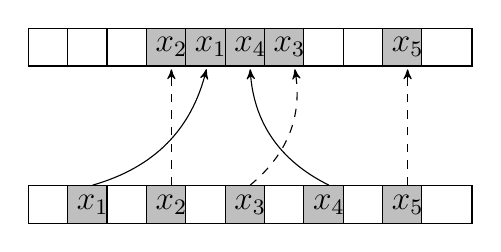
\begin{tikzpicture}[->,>=stealth',shorten >=1pt,auto,node distance=1cm,scale=.5,
  main node/.style={fill=white,rectangle,draw,font=\sffamily\large}]

  \node[main node,text=white] (0) at (1,4) {$x_2$};
  \node[main node,fill=gray!50] (1) at (2,4) {$x_1$};
  \node[main node,text=white] (2) at (3,4) {$x_2$};
  \node[main node,fill=gray!50] (3) at (4,4) {$x_2$};
  \node[main node,text=white] (4) at (5,4) {$x_2$};
  \node[main node,fill=gray!50] (5) at (6,4) {$x_3$};
  \node[main node,text=white] (6) at (7,4) {$x_2$};
  \node[main node,fill=gray!50] (7) at (8,4) {$x_4$};
  \node[main node,text=white] (8) at (9,4) {$x_2$};
  \node[main node,fill=gray!50] (9) at (10,4) {$x_5$};

  \node[main node,text=white] (10) at (11,4) {$x_2$};

  \node[main node,text=white] (12) at (1,8) {$x_2$};
  \node[main node,text=white] (13) at (2,8) {$x_1$};
  \node[main node,text=white] (14) at (3,8) {$x_2$};
  \node[main node,fill=gray!50] (15) at (4,8) {$x_2$};
  \node[main node,fill=gray!50] (16) at (5,8) {$x_1$};
  \node[main node,fill=gray!50] (17) at (6,8) {$x_4$};
  \node[main node,fill=gray!50] (18) at (7,8) {$x_3$};
  \node[main node,text=white] (19) at (8,8) {$x_4$};
  \node[main node,text=white] (20) at (9,8) {$x_2$};
  \node[main node,fill=gray!50] (21) at (10,8) {$x_5$};

  \node[main node,text=white] (22) at (11,8) {$x_2$};

  \path[every node/.style={font=\sffamily\tiny}]
    (1.north) edge [bend right] node {} (16)
    (7.north) edge [bend left] node {} (17)
    (5.north) edge [dashed, bend right] node {} (18)
    (3.north) edge [dashed] node {} (15)
    (9.north) edge [dashed] node {} (21)
;
\end{tikzpicture}
\caption{Example of a $N_2(\mathbf{L}_0)$-movement allowed by the CP model. Solid arrows correspond to elements that effectively changed their relative positions with respect to the remaining elements in the linear extension. Dashed arrows correspond to elements that maintained their positions, or only changed their absolute positions.}
\label{Movement}
\end{figure}

In order to account for the cost of having an incomparable pair $x_i, x_j \in \mathbf P$ adjacent in $\mathbf{L}_1$ with $V_i < V_j$, we shall write
\begin{eqnarray}
&& V_j - V_i \in \{1,2\} \Leftrightarrow B_{i,j},
\end{eqnarray}

\noindent where $B_{i,j}$ is a binary decision variable. We shall use variables $B_{i,j}$ to define an objective function, given by
\begin{eqnarray}
&& \sum_{\substack{i,j=1 \\ x_i \sim x_j}}^n c(x_i,x_j) B_{i,j}.
\end{eqnarray}

{\color{red}The trouble here is that we might have ``holes'' in the final sequence, consisting of two or more values from $\{1,\ldots,2n+1\}$ that are not taken by any $V_i$ ($i \in \{1,\ldots,n\}$). This breaks the strategy for keeping track of costs of ``adjacent'' pairs.\\


Moreover, if we end up with three consecutive elements in $\mathbf{L}_1$, then the model will incorrectly compute the total cost $c(\mathbf{L}_1)$.}\\

Additional/Redundant constraints:

\begin{eqnarray}
\sum_{\substack{j=1 \\ j \neq i}}^n B_{i,j} \leq 1, \; \forall i=1,\ldots,n
\end{eqnarray}

\section{Computational Results}

We embedded the CP model described in the previous section within a GRASP framework, in which a randomized version of Algorithm \ref{Liu2} is used as the constructive phase.

\section{Conclusions and Future Work}

Check the average improvement that we obtain by applying the CP local search to the solution produced by the randomized version of Liu2.\\

Compare the best solution obtained in this way with that obtained by running the deterministic version of Liu2.\\

Is the CP-based local search reasonable in terms of running time?

\end{document}